\documentclass{article}

\usepackage[utf8]{inputenc}
\usepackage{geometry}
\usepackage{graphicx}
\usepackage{titling}
\usepackage{fancyhdr}
\usepackage{cmbright}
\usepackage{caption}
\usepackage{subcaption}

\geometry{
	a4paper,
	total={170mm, 257mm},
	left=20mm,
	top=20mm
}


\title{Chapter 12 : Trains of Thought}
\author{Fharook Shaik}
\date{03 February 2025}

\fancypagestyle{fancy}{
	\fancyhf{}
	\fancyfoot[R]{
\includegraphics[width=3cm]{images/BTULogo_englisch_grau_2x.png}}
	\fancyfoot[L]{\thedate}
	\fancyhead[L]{13869 - Braitenberg Vehicle Praktium}
	\fancyhead[R]{\theauthor}
}

\pagestyle{fancy}

\makeatletter
\renewcommand{\maketitle}{
	\thispagestyle{fancy}
	\null
	\vskip 1em
	\begin{center}
		{\LARGE \@title \par}
	\end{center}
	\vskip 3em
}
\makeatother


\begin{document}

	\maketitle

	\noindent\begin{tabular}{@{}ll}
		Student & \theauthor\\
		Professor &  Dr. Cunningham, Douglas\\
		Matrikel-Nr.: & 5014962
		 
	\end{tabular}

	\section*{Summary}

	In Chapter 12, the narrative takes another significant step toward constructing vehicles that exhibit behaviors resembling true thinking. While previous vehicles could learn from experience, form associations, and predict future events based on past sequences, they lacked the ability to engage in sustained thought processes. Vehicle 12 introduces a mechanism that enables it to follow \textit{trains of thought} a sequence of mental states connected by logic, plausibility, or past experience.  

	At this point, the author acknowledges skepticism. While earlier vehicles have become increasingly sophisticated, adapting to their environment through both Darwinian selection and learned associations, they have yet to demonstrate anything that truly resembles thinking. Human thinking is characterized by long sequences of connected thoughts, the exploration of different possibilities, and the eventual arrival at conclusions. This chapter attempts to bridge that gap by designing a system that allows a vehicle to sustain a prolonged internal dialogue, reflecting on past experiences and reasoning through future possibilities.
	

	\subsection*{The Role of Threshold Control - Preventing Mental Overload}

	Before introducing thought processes, the chapter addresses a fundamental problem in advanced vehicles: the risk of \textit{epileptic overload}. Since associative learning strengthens connections between elements in the brain, excessive activation can trigger uncontrollable cascades of neural firing, leading to disorderly, ineffective behavior akin to epilepsy in biological brains. To prevent this, Vehicle 12 is equipped with a \textit{threshold control mechanism}.  

	Each element in the vehicle's brain is connected to a wire that adjusts its activation threshold. When brain activity is high, thresholds increase, making it harder for elements to activate. Conversely, when activity is low, thresholds decrease, allowing more elements to engage in processing. This self-regulating feedback loop ensures that the brain remains active without spiraling into chaotic overload.  

	The threshold control device plays a crucial role in stabilizing thought processes. When an external stimulus activates a concept within the brain, a controlled surge of activity follows. The threshold control mechanism quickly raises thresholds, suppressing most of the resulting activity while allowing the strongest, most relevant concept to remain active. This focusing effect mirrors what we observe in human cognition often described as the ability to focus attention.

	With attention focused on a single active concept, Vehicle 12 can now engage in a structured thought process. The key to this lies in the combination of two learning mechanisms:  


	\begin{enumerate}
		\item \textbf{Mnemotrix wires}, which form strong associative connections between elements that frequently activate together. These connections help establish stable, well-defined concepts.
		\item \textbf{Ergotrix wires}, which capture sequential relationships, linking concepts based on temporal order and causal relationships. 
	\end{enumerate}

	Once the threshold control system isolates an active concept, the Ergotrix wires trigger the next concept in the sequence. The process repeats as the threshold control suppresses weaker activations, allowing only the most consistent and familiar concepts to remain active. This mechanism creates a train of thought a continuous, structured progression of ideas, much like the way humans mentally navigate a city, predict chess moves, or debate consequences in an argument.  

	One critical feature of this system is its ability to avoid looping back to previous concepts, ensuring that thought remains dynamic and progressive. This self-sustaining mental activity is a hallmark of true thinking. Unlike previous vehicles that simply reacted to stimuli, Vehicle 12 can now explore possibilities internally, even without direct environmental input.  

	\begin{figure}[h]
		\centering
		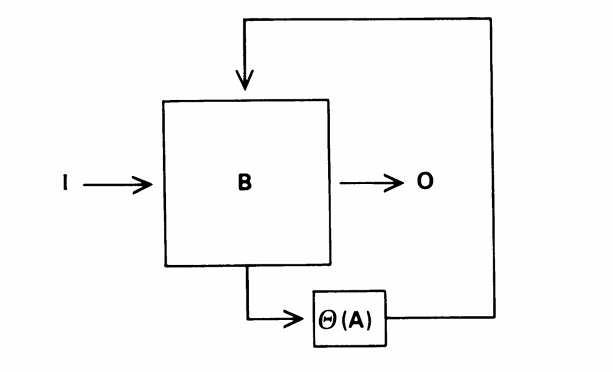
\includegraphics[scale=0.5]{images/figure-18.png}
		\caption{B is the brain, which receives input I and elaborates an output O.}
		\label{fig:vehicle-18}
	\end{figure}

	The chapter concludes with a bold philosophical claim: Vehicle 12 exhibits something very similar to free will. The author supports this by examining the unpredictability of its brain activity. Due to the threshold control mechanism, the number of active elements fluctuates in a complex, nonlinear manner. When plotted over time, these fluctuations form an unpredictable sequence.  

	From an observer's perspective, the vehicle's behavior becomes impossible to predict. Even though its brain operates on deterministic principles, no outside observer no matter how knowledgeable can foresee exactly what the vehicle will do at any given moment. Since predictability is often used as a measure of determinism, the inability to forecast Vehicle 12's actions suggests that it behaves as if it possesses \textit{free will}.  

	\begin{figure}[h]
		\centering
		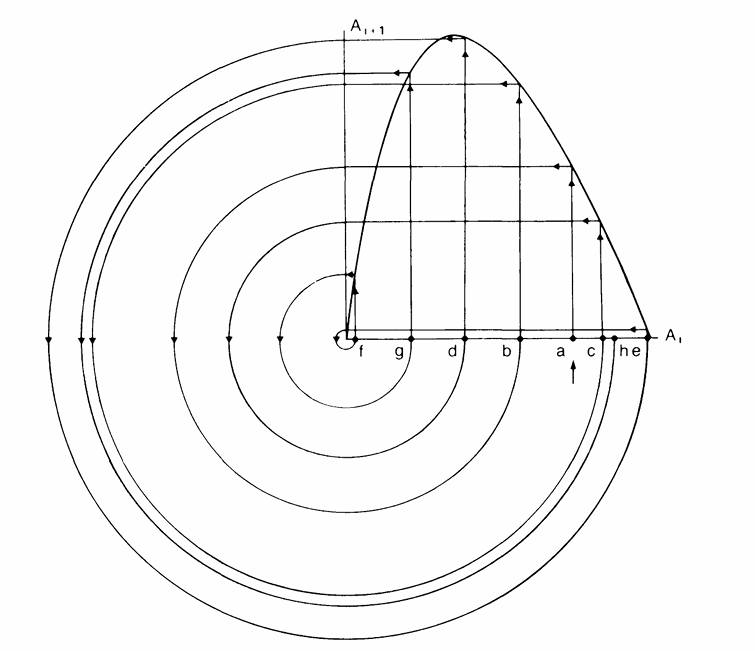
\includegraphics[scale=0.5]{images/figure-19.png}
		\caption{The function describing the next number of active elements A(i + 1) given the 
		present number of active elements A(i)}
		\label{fig:vehicle-19}
	\end{figure}

	The author anticipates objections from philosophers, who may argue that true free will requires an external decision-making force beyond any physical mechanism. However, he counters that if an entity behaves in every observable way as though it has free will, then for practical purposes, it does. The unpredictability of the vehicle's internal processes prevents external control or exploitation, reinforcing the subjective experience of autonomy.  


	\subsection*{Conclusion}
	
	Chapter 12 represents a major leap in the sophistication of artificial cognition. By integrating threshold control, associative learning, and sequential reasoning, Vehicle 12 is capable of sustaining complex trains of thought. This ability mirrors human cognition, where ideas unfold in a structured yet unpredictable manner.  

	Furthermore, the chapter introduces the provocative idea that unpredictability rather than an external, non-mechanical force can serve as a functional definition of free will. Whether or not this constitutes true autonomy, it is sufficient to create the illusion of independent decision-making.  

	With Vehicle 12, the line between machine and mind becomes increasingly blurred. As the series progresses, the final chapters will explore even more advanced aspects of intelligence, pushing synthetic psychology ever closer to the mysteries of human thought.  
\end{document}